\documentclass{article}
\usepackage[utf8]{inputenc}

\title{NTIN066 - Cache}
\author{Thuong-Hai Pham}
\date{December 2017}

\usepackage{graphicx}
\usepackage{amsmath}
\usepackage{amssymb}

\begin{document}

\maketitle

\section{Simulator}

\begin{figure}[h!]
\centering
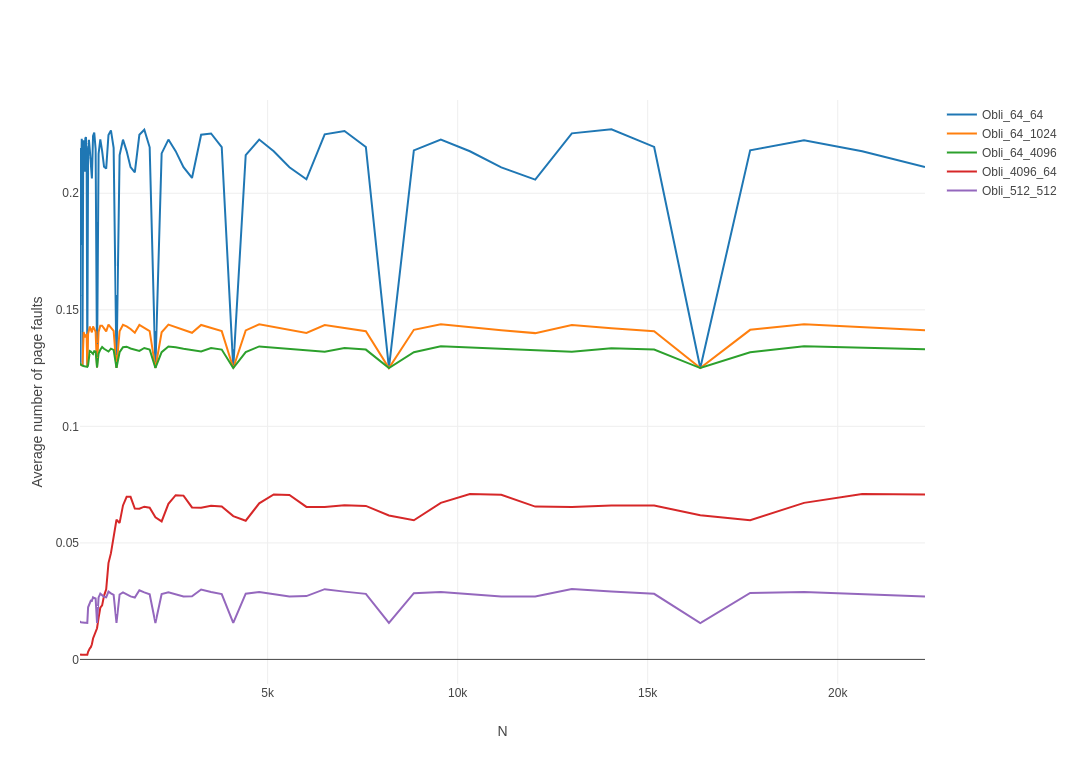
\includegraphics[width=\textwidth]{NTIN066-cache-data1.png}
\caption{Cache-oblivious algorithm with simulator}
\label{fig:plot1-obli}
\end{figure}

Figure \ref{fig:plot1-obli} shows the average number of page faults of the Cache-oblivious algorithm running with simulator. In general, the bigger size of a page B, the better result is due to z, the maximal size of a sub-matrix in the recursion that is fit into cache which $z\le B \le 2z$. To be precise, the average number of page faults is $O\left (10{\lceil \frac{N}{z} \rceil}^2 \frac{2z}{N^2-N}\right )$.

However, it is noted that the top three lines (Obli\_64\_64, Obli\_64\_1024, Obli\_64\_4096) has the same B value, yet different in results. At the point of $N=2^k=aB, a\in \mathbb{N}$, which matrix can be divided into $B\times B$ sub-matrices, the number of sub-matrices ${\lceil \frac{N}{B} \rceil}^2={\left ( \frac{N}{B} \right )}^2$ is at its minimum. Hence, the average number of page faults is $O(\frac{1}{B})$.

On the other hand, when $aB < N < (a+1)B, a\in \mathbb{N}$, the number of sub-matrices is higher. Therefore, the average number of page faults is constantly higher, and the bigger the cache is, the better.

The second strange behavior that does not obey the rule is Obli\_4096\_64. Although it has larger page size B, it does not hold the Tall-cache assumption, i.e. one matrix can not be fitted into the cache. Hence, the result is worse.

In addition, Obli\_4096\_64 only gets into constant line after $N=1024$, in which a row of size $4\times N$ bytes can not be fitted into one page.

\begin{figure}[h!]
\centering
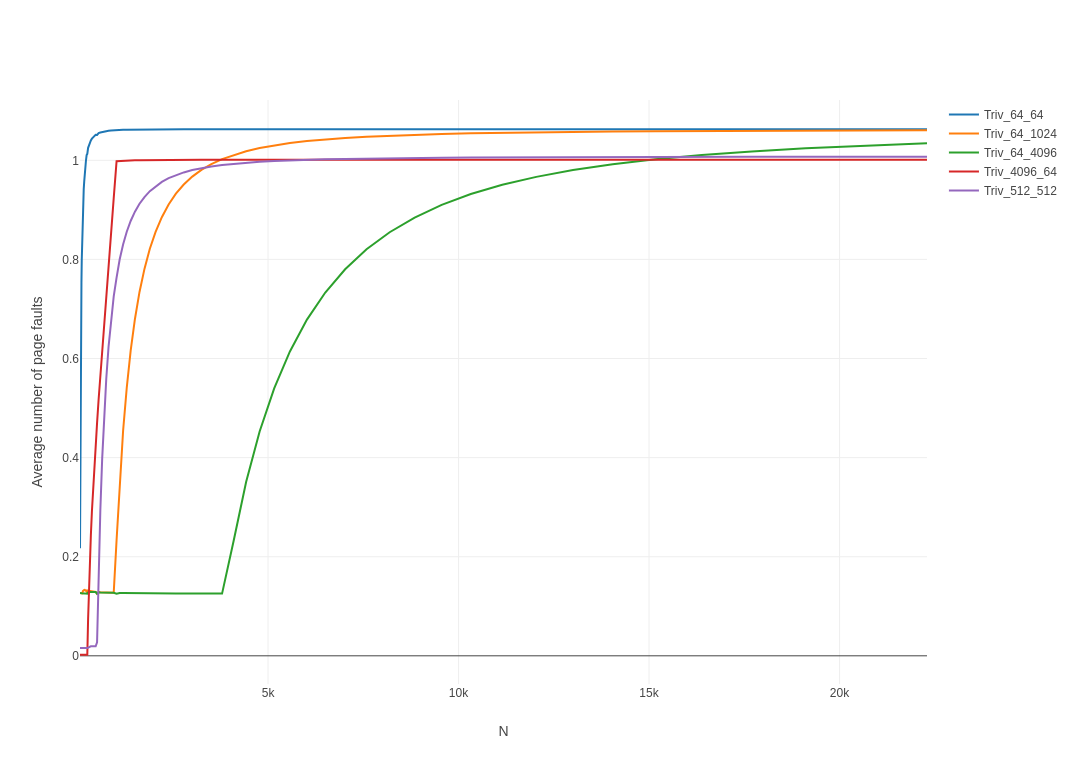
\includegraphics[width=\textwidth]{NTIN066-cache-plot1-triv.png}
\caption{Trivial algorithm with simulator}
\label{fig:plot1-triv}
\end{figure}

Figure \ref{fig:plot1-triv} shows that the trivial algorithm has the average number of page faults closer to 1, as expected. However, before N reaches the number of pages, the average number of page faults is closer to 0, because the whole matrix can be fitted into the cache.

\section{Real computer}
The real computer used in this experiment has an \textbf{Intel(R) Core(TM) i7-7700HQ CPU @ 2.80GHz} with \textbf{L1d cache: 32K, L1i cache: 32K, L2 cache: 256K, L3 cache: 8192K}.

\begin{figure}[h!]
\centering
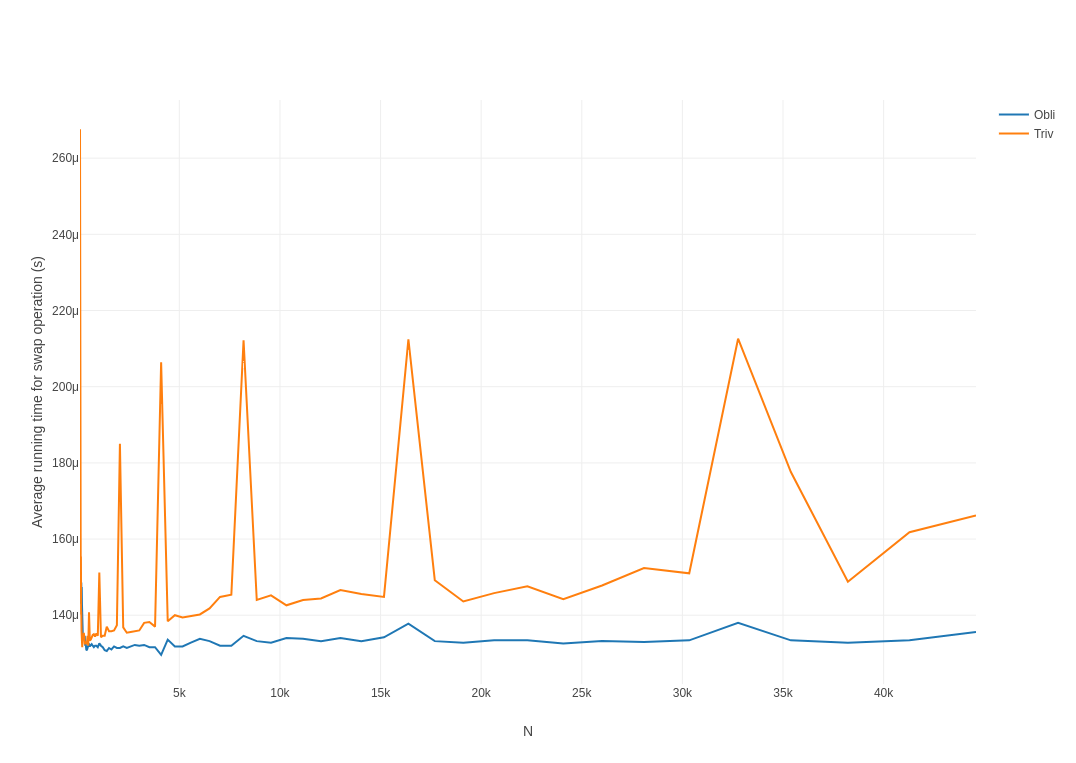
\includegraphics[width=\textwidth]{NTIN066-cache-plot2.png}
\caption{Trivial and Cache-oblivious algorithm on real computer}
\label{fig:plot2}
\end{figure}

Figure \ref{fig:plot2} shows the average of running time per swap operations for both algorithms. The numbers are average of 5 repeated experiments. It is obvious that Trivial algorithm takes longer time to do swap operation (proportional to the average number of page faults). However, in contrary to the idealized caches in Section 1, there are spikes at $N=2^k$ which means these N values produce more page faults. This is because the CPU uses set-associative cache instead of fully associative scheme as in our idealized caches.

\end{document}
